
\section{Introduction}

\subsection{Overview}

\begin{quote}
D3.2) Final field tested Integrated Energy System: Output of T3.1-5; Based on information provided by the deployment of deliverable 3.2 the software is further refined to provide energy services and community management (open source). 
\end{quote}

In the third year of Work Package 3 (WP3), we continued the design and development of the software platform YouPower\footnote{ \url{http://civis.tbm.tudelft.nl/}} expanding the results reported in D3.2. In this report, the final results are summarized as a whole for readability and usefulness. The refinement and improvement made in the third year are highlighted where necessary when possible. 
% 
The functionalities of the platform reported are deployed at Stockholm and Trento test sites respectively according to the local context. The YouPower software is open source under the Apache v.2 License\footnote{\url{https://github.com/CIVIS-project/YouPower/blob/master/LICENSE}}. It has  an online repository at GitHub\footnote{ \url{https://github.com/CIVIS-project/YouPower/}}. 
The backend API documentation is aslo available online\footnote{ \url{http://civis.tbm.tudelft.nl/apidoc/}}. 

...

%\subsection{Aims and Scope}

As stated in D3.2 \citep{Huang2015c}, the CIVIS platform is composed of two parts: the CIVIS back-end services, and the CIVIS front-end application with which users directly interact (Figure~\ref{fig:platform}). 
%
\begin{figure}
\begin{center}\footnotesize
	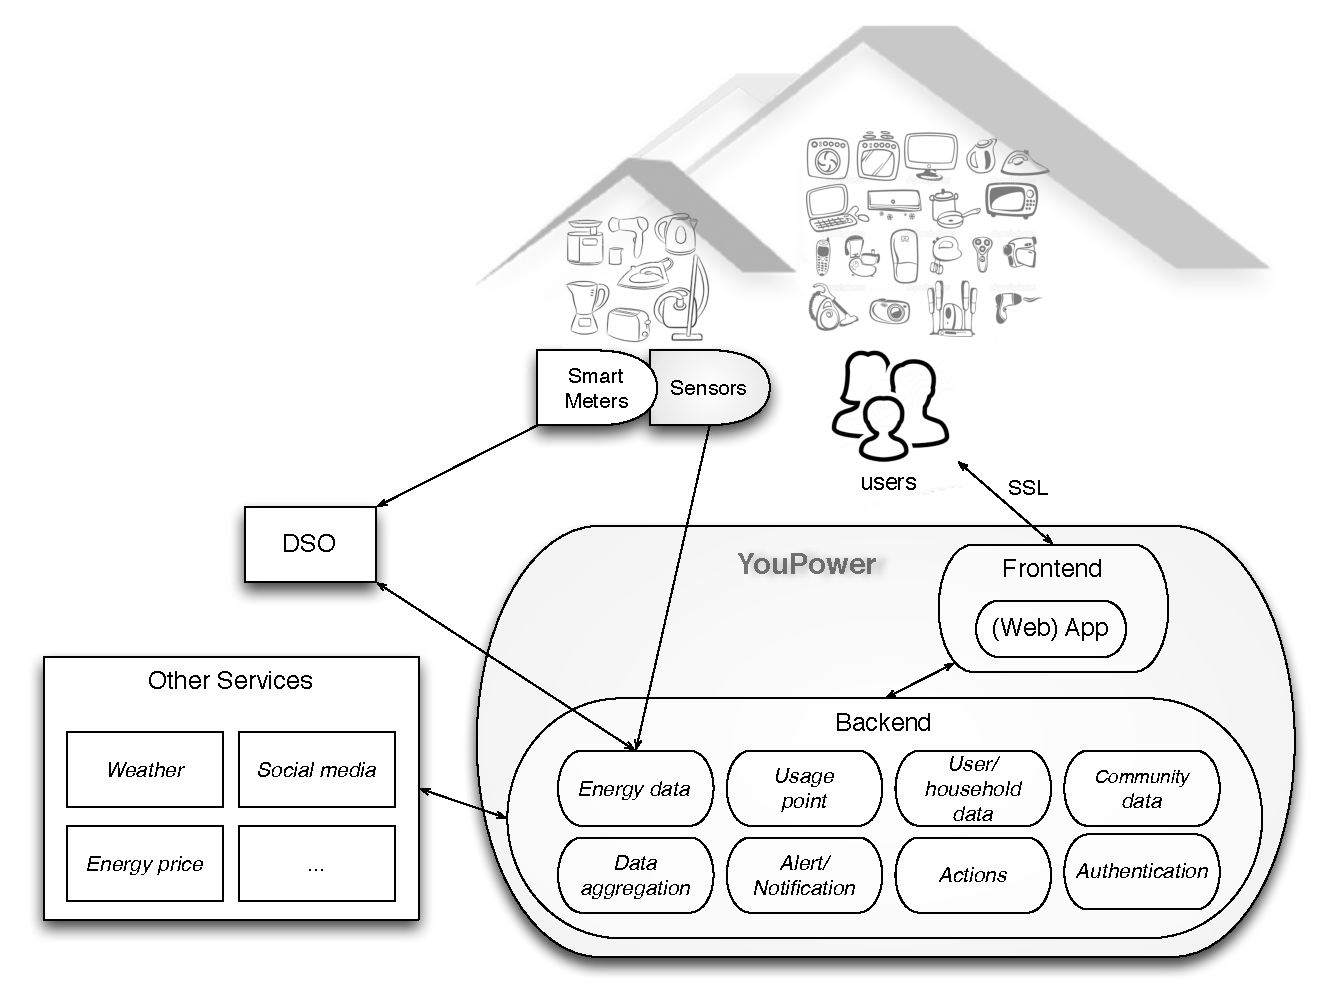
\includegraphics[width=.95\textwidth]{img/civis_platform_overview.pdf}\\
	DSO (Distribution System Operators),  SSL (Secure Sockets Layer)
	\caption{CIVIS platform overview}\label{fig:platform}
\end{center}
\end{figure}
% 
WP4 focuses on the system level ICT services that deal with energy data collected by smart meters and sensors at the Swedish and Italian test sites (see D4.3 for more details). 
WP3 focuses on the front-end application and the social level ICT services that deal with data related to user, household, community, action suggestions, etc. Unless otherwise specified, this report discusses the design and development of the WP3 part of the CIVIS platform which is called YouPower. (The CIVIS front-end application used to be called EnergyUP. The old name may be found in some old documents and/or mock-ups.)

... 

Environmental problems have their origins in human behavoir, and as a result, any solution to enviromental issues will require changes in behavoir 
\citep{Schultz2014}.
%The authentication of user sign up and login to an EnergyUP account is managed by WP3 services. A user may also choose to link his or her energy data, additional authentication is required. 

%The effectiveness of smart grids depends on consumer engagement and action. Today’s consumers have a vague understanding of the grid. How consumers understand the smart grid will shape how they feel about it, and in turn how readily they adopt it, and how they use it. 
%
%Seeing is believing 
%If consumers are given useful feedback on how they use energy and are provided with recommendations on how to improve, they will have the chances to make more informed energy choices. 
%
%

\subsection{Design and Development: the Continuation}

The design and development of YouPower is theory-driven, user-centered and iterative. We researched literature on intervention strategies and social smart grid applications directed at promoting pro-environmental consumer behavior change. This provided an initial set of design ideas that are iteratively refined and improved through the design process. Applying a user-centered design process can lead to more acceptable, satisfying and effective designs \citep{Brynjarsdottir2012}. This increases the potential of the intervention \citep{dick2012empowering} and may help increase user engagement with respect to the sense of relatedness to the application \citep{pierce2003state,schwartz2014people,edward2015review}. 

In the second year of CIVIS, we started with brainstorming sessions and a design workshop. A set of features was prototyped in simple handcrafted mock-ups used as a basis for discussion, and then underwent iterative rapid prototyping which produced wireframes as visual guides that can be more effectively communicated to general users. These prototypes were evaluated by user tests with groups of students and colleagues. Using the wireframe prototypes and later the software prototypes, we conducted focus group studies with consumers in Trento, test studies and focus groups with consumers and housing cooperative members in Stockholm, as well as a user study with pro-environmental participants in Helsinki. 

In the third year of CIVIS, the design and development continued. We have paid particular attention to quick responses to changes, and adaptive development. We also furthered literature research in environmental psychology and intervention design, and expanded the design guidelines based on our design practices and experiences. These guidelines can be useful for a wider group of designers interested in pro-environmental intervention.   .... >>>Any events in the third year?<<< ...   YouPower had been refined and improved gradually in the third year resulting in the current version of the application, which is deployed at Stockholm and Trento test sites. The rest of this report presents and discusses the latest version of YouPower. 

%literature, group feedback (internal), user feedback: workshops, focus groups 
 
